%%%%%%%%%%%%%%%%%%%%%%%%%%%%%%%%%%%%%
% Document properties and packages
%%%%%%%%%%%%%%%%%%%%%%%%%%%%%%%%%%%%%
\documentclass[a4paper,11pt,final]{memoir}
\usepackage{CJKutf8}%中文支持

% misc
\renewcommand{\familydefault}{bch}	% font
\pagestyle{empty}					% no pagenumbering
\setlength{\parindent}{0pt}			% no paragraph indentation
% required packages (add your own)
\usepackage{flowfram}% column layou
\usepackage{marvosym}
\usepackage{textcomp}

\usepackage[top=1cm,left=1cm,right=1cm,bottom=1cm]{geometry}% margins
\usepackage{graphicx}										% figures
\usepackage{hyperref}
\definecolor{linkcolour}{rgb}{0,0.2,0.6}  %蓝色
\hypersetup{colorlinks,breaklinks,urlcolor=linkcolour, linkcolor=linkcolour}										% URLs
\usepackage[usenames,dvipsnames]{xcolor}					% color
\usepackage{multicol}										% columns env.
	\setlength{\multicolsep}{0pt}
\usepackage{paralist}										% compact lists
\usepackage{tikz}

%%%%%%%%%%%%%%%%%%%%%%%%%%%%%%%%%%%%%
% Create column layout
%%%%%%%%%%%%%%%%%%%%%%%%%%%%%%%%%%%%%
% define length commands
\setlength{\vcolumnsep}{\baselineskip}
\setlength{\columnsep}{\vcolumnsep}
%定义主题颜色,可选颜色 Maroon,ForestGreen,DarkOrchid,RoyalBlue,Turquoise,Cyan,etc,更多颜色参考xcolor包的颜色定义
\newcommand{\myThemeColor}{RoyalBlue}
% frame setup (flowfram package)
% left frame
\newflowframe{0.23\textwidth}{\textheight}{0pt}{0pt}[left]
	\newlength{\LeftMainSep}
	\setlength{\LeftMainSep}{0.23\textwidth}
	\addtolength{\LeftMainSep}{1\columnsep}
 
% small static frame for the vertical line
\newstaticframe{1.5pt}{\textheight}{\LeftMainSep}{0pt}
 
% content of the static frame
\begin{staticcontents}{1} %绘制分割线
\hfill
\tikz{%
	\draw[loosely dotted,color=\myThemeColor,line width=1.5pt,yshift=0]
	(0,0) -- (0,\textheight);}%
\hfill\mbox{}
\end{staticcontents}
 
% right frame
\addtolength{\LeftMainSep}{1.5pt}
\addtolength{\LeftMainSep}{1\columnsep}
\newflowframe{0.7\textwidth}{\textheight}{\LeftMainSep}{0pt}[main01]


%%%%%%%%%%%%%%%%%%%%%%%%%%%%%%%%%%%%%
% define macros (for convience)
%%%%%%%%%%%%%%%%%%%%%%%%%%%%%%%%%%%%%
\newcommand{\Sep}{\vspace{1em}}
\newcommand{\SmallSep}{\vspace{0.9em}}

\newenvironment{AboutMe}
	{\ignorespaces\textbf{\color{\myThemeColor} About me}}
	{\Sep\ignorespacesafterend}
%定义 section	
\newcommand{\CVSection}[1]
	{\Large\textbf{#1}\par
	\vspace{0.2cm}\normalsize\normalfont}

\newcommand{\CVItem}[1]
	{\textbf{\color{\myThemeColor} #1}}


%%%%%%%%%%%%%%%%%%%%%%%%%%%%%%%%%%%%%
% Begin document
%%%%%%%%%%%%%%%%%%%%%%%%%%%%%%%%%%%%%
\begin{document}

\begin{CJK*}{UTF8}{gbsn}%选择字体,黑体
% Left frame 左边内容在此定义
%%%%%%%%%%%%%%%%%%%%
\begin{figure}
	\hfill
	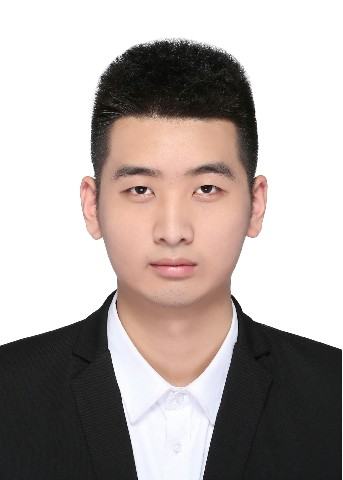
\includegraphics[width=0.9\columnwidth]{avatar1}
	\vspace{-7cm}
\end{figure}
\begin{flushright}\footnotesize
.\\
\vskip 6cm
    \raggedright
	\CVItem{{\large 个人信息:}}\\
	\textbf{电子邮件:}\\
	\href{mailto:yingpengma@gmail.com}{yingpengma@gmail.com}  \\
	\textbf{个人主页 \& Blog:}\\
	\href{https://ingingx.xyz/}{https://ingingx.xyz/}\\
	\textbf{手机:}\\
	+86 - 15108482982\\
	\textbf{政治面貌:}\\
	党员

		
	\CVItem{{\large 语言能力:}}\\
	\textit{\textbf{英语}:\\
		    ~~IELTS: 7.0\\
		    ~~GRE: 319+3.0\\
		    ~~四级、六级:通过\\
		   \textbf{中文}:母语 \\ 
		   \textbf{德语}:简单沟通
			}
	
	\CVItem{{\large 电脑技能:}}\\
	$\bullet$\textbf{编程语言:}\\ C/C++, MATLAB, Python, Java, HTML5, 汇编 \\
	$\bullet$\textbf{工作软件:}\\ VS, MATLAB, Sypder3, PyTorch \\
	$\bullet$\textbf{科学计算:}\\ MATLAB, PyNum
	

	\CVItem{ }\\
	\textbf{关于:}\\ 11223344 \\


\end{flushright}\normalsize
\framebreak


% Right frame 右边内容在此定义
%%%%%%%%%%%%%%%%%%%%%
\Huge\bfseries {\color{\myThemeColor} 马~瀛~鹏~~MA, Yingpeng}\\
\normalsize\normalfont

% Education
\CVSection{教育背景}
\hrule
\SmallSep
\CVItem{2019.09 - Present\hfill\textsc{Gap Year\footnote{已获南卡罗莱纳大学 (\href{https://sc.edu/}{UofSC}) Ph.D. offer (fall 2019),因故放弃,目前在申请欧洲硕士课程 (fall/winter 2020)},四川成都}}\\
\textit{-独立开发、仿真项目}
\\
\CVItem{2017.08 - 2019.06\hfill\textsc{图像处理研究所~IoIP,电子科技大学}}\\
\textit{-研究助理}
\\
\CVItem{2015.09 - 2019.06\hfill\textsc{电子科技大学~UESTC,四川成都}}\\
\textit{-信息与通信工程学院 \quad 通信工程学士 (B.Eng. of Comm.)}
\\
\CVItem{2016.08 - 2016.09\hfill\textsc{新加坡国立大学~NUS,新加坡}}\\
\textit{-暑假课程}
\\


% Experience
\CVSection{实习经历}
\hrule
\SmallSep
\CVItem{2017.08 - 2017.09 \hfill 大唐电信,成都}\\
\textit{$\bullet$ 实习研究助理,初始化电信基站,研究交换算法(Dijkstra)并仿真}
\\
\CVItem{2016.09 - 2016.10 \hfill 创青春大赛,电子科技大学}\\
\textit{$\bullet$ 担任志愿者,指引参赛学生出入场,维护赛场秩序}
\\
\CVItem{2016.08 - 2016.09 \hfill ERA,新加坡}\\
\textit{$\bullet$ 市场调查,调研新加坡市场对房地产的价格需求。获“优秀实习生推荐信”} 
\\
\CVItem{2015.09 - 2015.12\hfill Syslab,电子科技大学}\\
\textit{$\bullet$ 实习开发员,与组员一同完成简单app的开发(基于Android 2.x)}
\\
\CVItem{2015.09 - 2016.06\hfill 通信学院学生会,电子科技大学}\\
\textit{$\bullet$ 担任“新青年”部员,策划并参与“荧光夜跑”、“迎新晚会”等多场活动}
\\
\CVItem{2015.09 - 2016.06\hfill 班长,电子科技大学}\\
\textit{$\bullet$ 负责班级管理,组织班级活动,与同学建立良好友谊}
\\

% CAMPU
\CVSection{科研经历}
\hrule
\SmallSep
\CVItem{2019.10,CEEMD 与 LSSVM 的数据预测 \hfill \emph{Researcher}}\\
\textit{$\bullet$ 利用 Python 中 Pandas 将原始数据从 HTML 转换为 EXCEL;应用 CEEMD 分解数据,并用 LSSVM 预测之后的趋势} 
\\
\CVItem{2019.09,MSK 与多普勒频移的通信系统仿真与优化 \hfill \emph{Researcher}}\\
\textit{$\bullet$ 在 Simulink 平台搭建 MSK 通信系统,并引入 Doppler Shift 以模拟实际通信信道;结合信道估计与导频技术对其优化,对比误码率} 
\\
\CVItem{2017.09 - 2019.06,基于Bitmap的显著性探索 \hfill \emph{Researcher}}\\
\textit{$\bullet$ 分析图像 Bitmap 以及编码信息,作为预处理步骤,尝试改进已有显著性检测方案。目前团队力图改进该方案,使之可以作为绝大多数已有显著性检测模型的增强方法} 
\\
\CVItem{2017.12 - 2018.03, 基于 Bitplane Slicing 的显著性检测 \hfill \emph{Leader}}\\
\textit{$\bullet$ 分析图像 Bitplane Slicing 信息,总结可利用内容,构建脱离深度学习框架的图片显著性检测模型,并在大量数据集上测试,对比先进模型,提出不足与改进方案。该项目参与“2018年大学生创新创业项目”,完成答辩,并获“\textbf{A}”评价} 
\\
\CVItem{2018.05 - 2018.07, SIMO系统性能仿真分析 \hfill \emph{Leader}}\\
\textit{$\bullet$ 学习了解 SIMO 与大规模 MIMO 技术,利用 MATLAB与 SIMILINK 对其仿真} 
\\
\CVItem{2017.11 - 2018.03, 基于AUX的信息传输 \hfill \emph{Leader}}\\
\textit{$\bullet$ 利用AUX音频传输线,设计调制解调模块与编码方案,在两台电脑之间实现图片、音频、文字传输}
\\

% HONORS & SCHOLARSHIPS
\CVSection{个人荣誉}
\hrule
\SmallSep
	\begin{tabular}{l|l}
		$\Rightarrow$ 2016&\textit{电子科技大学社会实践优秀个人}\footnotesize\\
		$\Rightarrow$ 2016&\textit{电子科技大学数学竞赛三等奖}\\
	\end{tabular}

%%%%%%%%%%%%%%%%%%%%%%%%%%%%%%%%%%%%%
% End document
%%%%%%%%%%%%%%%%%%%%%%%%%%%%%%%%%%%%%
\end{CJK*}
\end{document}